\documentclass{beamer}
\usepackage{minted}
\usepackage{epigraph}
\usepackage{subfig}
\usepackage{pgfplots}
\usepackage{tikz}
\usepackage{color, colortbl}

\usetheme{focus}

\definecolor{orangered}{rgb}{1,0.45, 0}

\title{Shell Linux \& BASH scripting}
\subtitle{Tutorato Sistemi Operativi}
\author{Davide Carnemolla}
\titlegraphic{
\includegraphics[scale=0.13]{images/penguin2.pdf}}
\institute{Dipartimento di Matematica e Informatica \\ Università di Catania}
\date{2022/2023}

\begin{document}
    \begin{frame}
        \maketitle
    \end{frame}

    \begin{frame}{> whoami}
        
    \end{frame}
    
    \section{Shell Linux}

    \begin{frame}{La Shell}
        \begin{columns}[t, onlytextwidth]
            \column{0.2\textwidth}
                \centering
                
\includegraphics[height=2.5cm, keepaspectratio]{images/user.pdf}

            \column{0.2\textwidth}
                \centering
                
\includegraphics[height=2cm, keepaspectratio]{images/rightarrow.pdf}
            
            \column{0.2\textwidth}
                \centering
                
\includegraphics[height=2.5cm,keepaspectratio]{images/terminal.pdf}

            \column{0.2\textwidth}
                \centering
                
\includegraphics[height=2cm, keepaspectratio]{images/rightarrow.pdf}

            \column{0.2\textwidth}
                \centering
                
\includegraphics[height=2.5cm, keepaspectratio]{images/linux.pdf}
        \end{columns}
    \end{frame}

    \begin{frame}{Il filesystem}
        \centering
        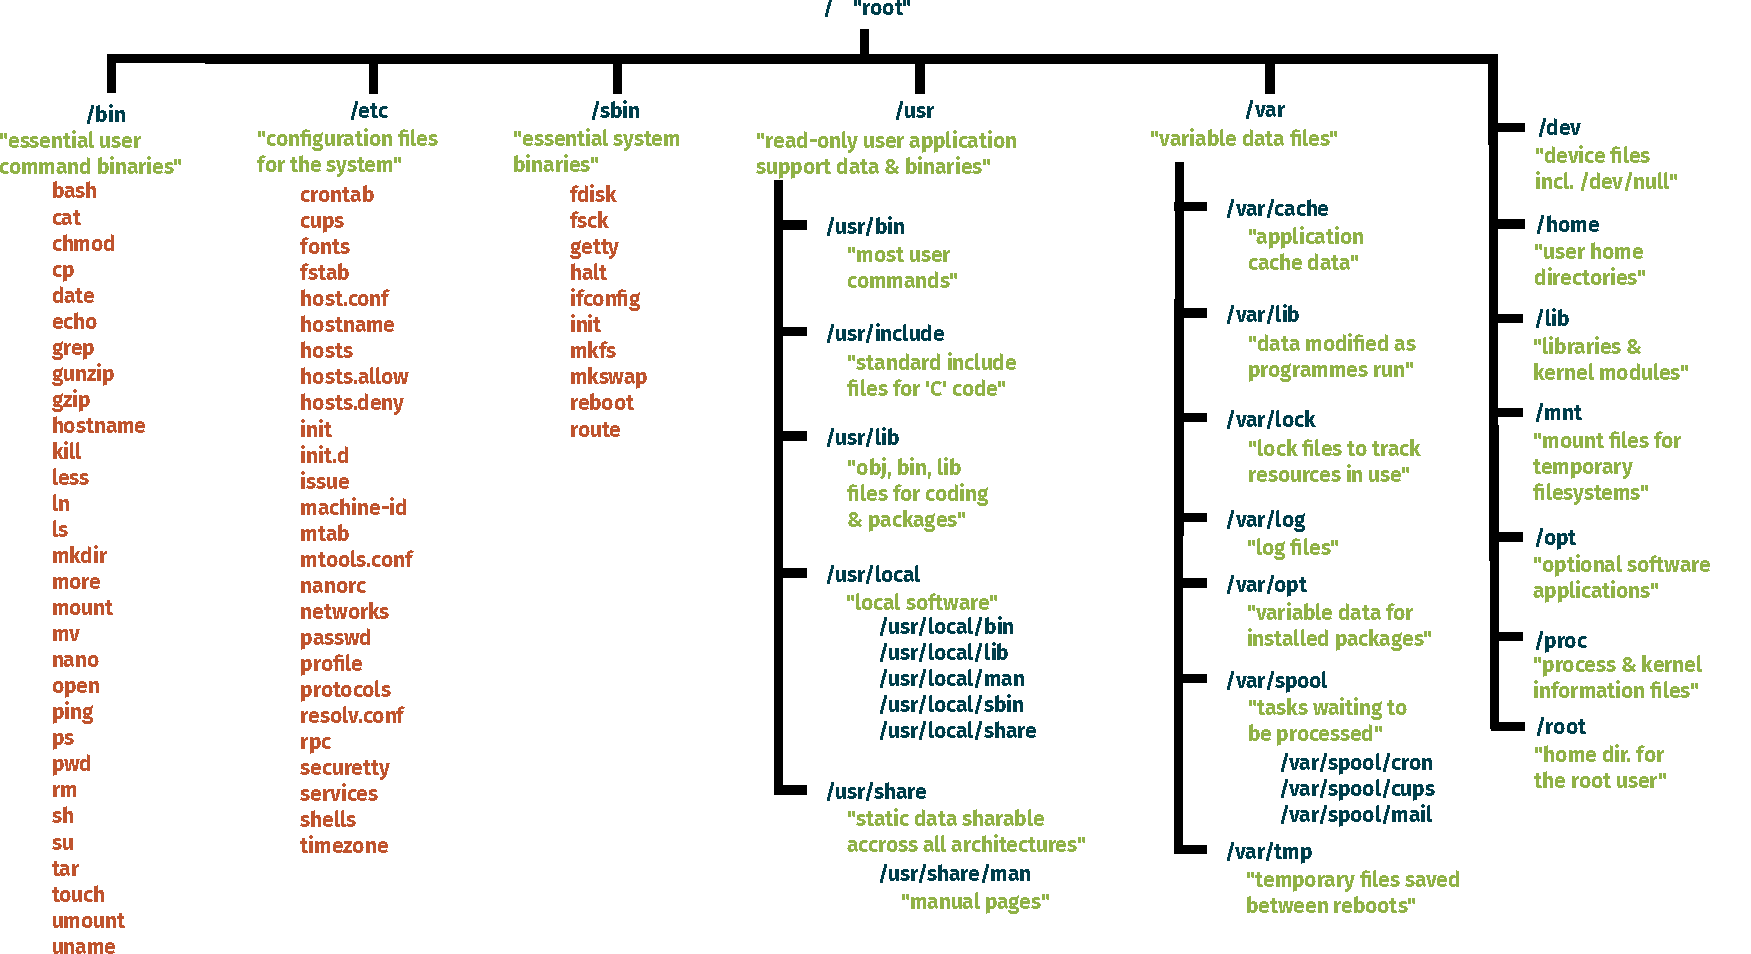
\includegraphics[height=6cm, keepaspectratio]{images/unix-fs.pdf}
    \end{frame}

    \begin{frame}{I Path}
        \centering
        
\includegraphics[height=2cm, keepaspectratio]{images/path.pdf}
        \vspace{0.5cm}
        \begin{block}{Path assoluto}
            Il \textbf{percorso assoluto} di un file è il percorso
            che va dalla radice del filesystem allo stesso.
        \end{block}

        \begin{block}{Path relativo}
            Fissando logicamente una particolare directory (in genere quella corrente) è possibile identificare un file attraverso il
            \textbf{percorso relativo} che va da tale directory ad esso.
        \end{block}
    \end{frame}

    \begin{frame}{I Path}
        \begin{alertblock}{Nota}
            Il percorso assoluto di un file è il suo percorso relativo rispetto
            alla root.
        \end{alertblock}

        \begin{exampleblock}{Esempio}
            \textbf{Directory corrente}: \textit{/home/}

            \textbf{Path assoluto}: \textit{/home/davide/file.txt}

            \textbf{Path relativo}: \textit{davide/file.txt}
        \end{exampleblock}

        \begin{block}{Cartelle virtuali}
            \begin{itemize}
                \item la cartella \textit{.} indica la cartella stessa
                \item la cartella \textit{..} indica la cartella genitore (utile per navigare il filesystem)
            \end{itemize}
        \end{block}
    \end{frame}

    \begin{frame}{Path: file di dispositivo}
        In ambiente UNIX esistono dei file speciali chiamati file di dispositivo:
        identificano una particolare periferica del sistema ed attraverso questo è possibile interagire con tale periferica. \\
        \vspace{0.25cm}
        \begin{columns}[t, onlytextwidth]
            \column{0.5\textwidth}
                \centering
                
\includegraphics[height=1.5cm, keepaspectratio]{images/char.pdf}
                
                \textbf{A caratteri}

            \column{0.5\textwidth}
                \centering
                
\includegraphics[height=1.5cm, keepaspectratio]{images/block.pdf}
                
                \textbf{A blocchi}
        \end{columns}

        \vspace{0.25cm}

        \begin{exampleblock}{Esempi}
            \begin{itemize}
                \item \textit{/dev/sda,/dev/sdb}\dots
                \item \textit{/dev/sda1,/dev/sda2}\dots
                \item \textit{/dev/tty1,/dev/tty2}\dots
            \end{itemize}
        \end{exampleblock}
    \end{frame}

    \begin{frame}{Mount: quando voglio più spazio}
        \centering
        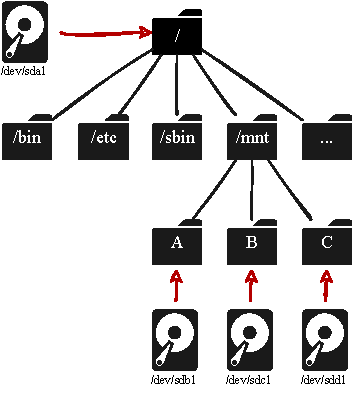
\includegraphics[height=7.5cm, keepaspectratio]{images/mountpoint.pdf}
    \end{frame}

    \begin{frame}{Hello Shell}
        \begin{exampleblock}{}
            \$ echo "Hello shell" 
        \end{exampleblock}

        \begin{itemize}
            \item \textbf{echo} rappresenta il comando
            \item \textbf{"Hello world"} rappresenta un parametro per il comando
        \end{itemize}

        \begin{block}{Parametri}
            Tipicamente un comando può richiedere dei parametri
            
            \vspace{0.5cm}

            \begin{columns}[t, onlytextwidth]
                \column{0.33\textwidth}
                    \centering
                    
\includegraphics[height=1cm, keepaspectratio]{images/file.pdf}
                    
                    \textbf{File}
    
                \column{0.33\textwidth}
                    \centering
                    
\includegraphics[height=1cm, keepaspectratio]{images/input-data.pdf}
                    
                    \textbf{Dati}
                \column{0.33\textwidth}
                    \centering
                    
\includegraphics[height=1cm, keepaspectratio]{images/options.pdf}
                    
                    \textbf{Opzioni}
            \end{columns}

            \vspace{0.5cm}
        \end{block}
    \end{frame}

    \begin{frame}{Hello Shell: comandi utili}
        \begin{columns}[t, onlytextwidth]
            \column{0.33\textwidth}
                \centering
                \Huge \textbf{CTRL + C}
                
                \vspace{0.2cm}
                
                \normalsize \textit{``No maria, io esco''}
            \column{0.33\textwidth}
                \centering
                \Huge \textbf{CTRL + S}

                \vspace{0.2cm}

                \normalsize \textit{``Finisco di mangiare la peperonata e scendo! ''}
            \column{0.33\textwidth}
                \centering
                \Huge \textbf{CTRL + Q}

                \vspace{0.2cm}

                \normalsize \textit{``Va bene, fammi vedere qualcosa''}
        \end{columns}
    \end{frame}

    \begin{frame}{Hello man}
        \begin{columns}[t, onlytextwidth]
            \column{0.33\textwidth}
                \centering
                
\includegraphics[height=2cm]{images/search.pdf}

                \vspace{0.2cm}

                \textit{apropos stringa}
            \column{0.33\textwidth}
                \centering
                
\includegraphics[height=2cm]{images/whatis.pdf}

                \vspace{0.2cm}

                \textit{whatis stringa}
            \column{0.33\textwidth}
                \centering
                
\includegraphics[height=2cm]{images/man.pdf}

                \vspace{0.2cm}
                
                \textit{man stringa}
        \end{columns}
    \end{frame}

    \begin{frame}{Navigare il filesystem: ls}
    \end{frame}

    \section{BASH}
    
\end{document}
